%
% file : learn_git.tex
% date : jeudi 19 décembre 2019, 13:19:09 (UTC+0100)
% author : sedelpeuch
% description :
\documentclass[a4paper,10pt]{article}
\usepackage[utf8]{inputenc}
\usepackage[T1]{fontenc}
\usepackage[french]{babel}
\usepackage{graphicx}
\usepackage{float}
\usepackage{amsmath}
\usepackage{amssymb}
\usepackage{mathrsfs}
\usepackage{color}
\usepackage{fancyhdr}
\usepackage{pdfpages}
\usepackage{layout}
\usepackage{multicol}
\usepackage{setspace}
\usepackage{csvsimple}
\usepackage[table]{xcolor}
\usepackage[colorlinks=true]{hyperref}
\usepackage{tikz, tkz-tab}
\usepackage[top=2cm,bottom=2cm,left=2cm,right=2cm]{geometry}
\usepackage{amsthm}
\usepackage{listings}
\setlength{\parindent}{0cm}
\setlength{\parskip}{1ex plus 0.5ex minus 0.2ex}
\newcommand{\hsp}{\hspace{20pt}}
\newcommand{\HRule}{\rule{\linewidth}{0.1mm}}

\definecolor{darkWhite}{rgb}{0.94,0.94,0.94}

\lstset{
  backgroundcolor=\color{darkWhite},
  basicstyle=\footnotesize,
  captionpos=b,
  commentstyle=\color{red},
  deletekeywords={...},
  escapeinside={\%*}{*)},
  extendedchars=false,
  keepspaces=false,
  keywordstyle=\color{blue},
  language=bash,
  literate=
  {²}{{\textsuperscript{2}}}1
  {⁴}{{\textsuperscript{4}}}1
  {⁶}{{\textsuperscript{6}}}1
  {⁸}{{\textsuperscript{8}}}1
  {€}{{\euro{}}}1
  {é}{{\'e}}1
  {è}{{\`{e}}}1
  {ê}{{\^{e}}}1
  {ë}{{\¨{e}}}1
  {É}{{\'{E}}}1
  {Ê}{{\^{E}}}1
  {û}{{\^{u}}}1
  {ù}{{\`{u}}}1
  {â}{{\^{a}}}1
  {à}{{\`{a}}}1
  {á}{{\'{a}}}1
  {ã}{{\~{a}}}1
  {Á}{{\'{A}}}1
  {Â}{{\^{A}}}1
  {Ã}{{\~{A}}}1
  {ç}{{\c{c}}}1
  {Ç}{{\c{C}}}1
  {õ}{{\~{o}}}1
  {ó}{{\'{o}}}1
  {ô}{{\^{o}}}1
  {Õ}{{\~{O}}}1
  {Ó}{{\'{O}}}1
  {Ô}{{\^{O}}}1
  {î}{{\^{i}}}1
  {Î}{{\^{I}}}1
  {í}{{\'{i}}}1
  {Í}{{\~{Í}}}1,
  morekeywords={*,...},
  showspaces=false,
  showstringspaces=false,
  showtabs=false,
  stepnumber=1,
  tabsize=4,
}
\begin{document}
\begin{spacing}{1.5}
\graphicspath{{image/}}
\setcounter{tocdepth}{2}
\newpage
\pagestyle{fancy} \lhead{} \chead{\textbf{Guide de survie Github}}
\rhead{\thepage} \lfoot{} \cfoot{} \fancyfoot[R] {
  
\includegraphics[scale=0.075]{65508.png} }
\HRule
\begin{center}
  \LARGE \textbf{Guide de survie pour Git}
\end{center}
\HRule \\

\subsection*{Github, qu'est ce que c'est ?}
Github est un service en ligne qui permet d'héberger ses repositories de code.
Github est un outil gratuit pour héberger du code open source.
Pour commencer à utiliser Github il faut créer son compte sur la page
\href{https://github.com/join?source=header-home}{page d'acceuil}, rentrer son
nom d'utilisateur , un mot de passe etc. Une fois cela fait, il faut
penser à communiquer son pseudo pour pouvoir accéder au dossier d'eirbot. \\
Sur Linux il suffit d'avoir un terminal pour faire toutes les commandes git. En
revanche si vous êtes sur Windows...tant pis\footnote{L'utilisation de logiciel
  comme \href{https://gitforwindows.org/}{Git SCM} permettra de réaliser toutes
  les actions après chacun peut utiliser son logiciel préféré, vive \textsc{emacs}}

\subsection*{Récupérer du code d'un autre d'un autre repository}
Une fois le compte Github créé, du code d'un autre
repository peut être récupéré. Pour cela il faut \textbf{cloner} le répertoire,
il suffit de cliquer sur ``clone'' sur Github et de copier le lien en https. (On
pourra modifier pour pouvoir utiliser le ssh plus tard).
\begin{figure}[H]
  \center
  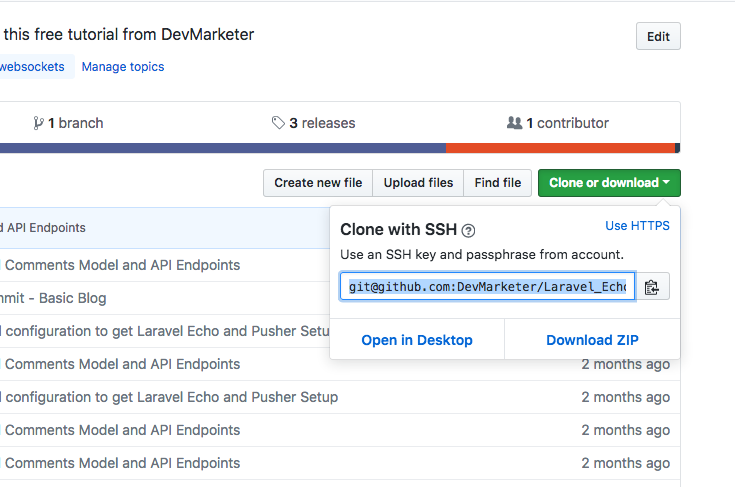
\includegraphics[scale=0.5]{clone.png}
\end{figure}
Une fois le lien copié on tape dans un bash la commande suivante
\begin{center}
  \begin{tabular}{c}
    \rowcolor{lightgray!50!white}
      \textbf{git clone} https://github.com/eirbot/eirbot2020-1A.git
  \end{tabular}
\end{center}
Cela permet de créér une copie locale du dossier sur notre machine.

\subsection*{Envoyer du code sur Github}
Maintenant qu'une copie locale du dossier existe sur la machine, le code (ou
n'importe quel fichier) peut être modifié de manière locale. Lorsque le travail
terminé il faut synchroniser les modifications effectuées sur le repository
local avec le repository distant. L'opération que nous allons décrire permet de valider un
ensemble de modifications dans le code pour créer une nouvelle révision, et est
communément appelé un \textbf{commit}.\\
Commençons par visualiser l'état des fichiers dans le dépôt avec la commande
suivante\footnote{Cette étape est assez pratique au début pour comprendre où
  l'on va, on s'en passe rapidement}
\begin{center}
  \begin{tabular}{c}
    \rowcolor{lightgray!50!white}
      \textbf{git status}
  \end{tabular}
\end{center}
Si le fichier n'a jamais été communiqué au dépôt, le résultat devrait être être
de la forme
\begin{lstlisting}
Untracked files:
  (use "git add <file>..." to include in what will be committed)

      nom_du_fichier
\end{lstlisting}
Si le fichier était déjà présent dans le dépôt, le résultat devrait être de la
forme  :
\begin{lstlisting}
Changes not staged for commit:
  (use "git add <file>..." to update what will be committed)
  (use "git checkout -- <file>..." to discard changes in working directory)

    modified:   nom_du_fichier
\end{lstlisting}
Une fois que nous connaissons l'état des fichiers il faut choisir ceux que l'on veut envoyer
pour cela
\begin{center}
  \begin{tabular}{c}
    \rowcolor{lightgray!50!white}
      \textbf{git add} nom\_du\_fichier
  \end{tabular}
\end{center}
Une fois les fichiers ajouté nous pouvons \textbf{commit} ces derniers via
\begin{center}
  \begin{tabular}{c}
    \rowcolor{lightgray!50!white}
      \textbf{git commit}
  \end{tabular}
\end{center}
Cela va ouvrir un éditeur de texte, il faut ajouter un commentaire. Une fois le
commentaire validé la révision a été créé.\\ \textcolor{red}{Attention !} Les
commentaires des commits sont les premières choses que les collaborateurs vont
voir, un commit comme ``pause dej'' n'a aucun intéret\footnote{Cela a plutôt
  tendance à énerver vos collègues et les conduire à détruire chaqu'un de vos
  commits (oui oui c'est possible)}, les collaborateurs ne peuvent pas
comprendre ce que vous avez fait. Il est donc conseillé de commit fichier par
fichier en expliquant correctement les modifications réalisées sur chaque
fichier.\\
Comme il s'agit d'une modification des sources, il faut la communiquer au dépôt
distant. Le dépôt distant se nomme par défaut origin, et la branche à
communiquer master. Communiquer votre modification des sources avec la commande
suivante :
\begin{center}
  \begin{tabular}{c}
    \rowcolor{lightgray!50!white}
      \textbf{git push} origin master
  \end{tabular}
\end{center}

\newpage
\subsection*{Récupérer des modifications}
Pour récupérer en local les dernières modifications du repository Github, il
faut utiliser la commande la commande
\begin{center}
  \begin{tabular}{c}
    \rowcolor{lightgray!50!white}
      \textbf{git pull} origin master
  \end{tabular}
\end{center}
Lorsque l'on réalise un \textbf{git pull} on effectue un fetch puis
un merge. Dans nos conditions de travail, il est préférable de
réaliser un rebase pour que cela soit automatique il faut taper la commande
suivante.
\begin{center}
  \begin{tabular}{c}
    \rowcolor{lightgray!50!white}
      git config - - global branch.master.rebase true
  \end{tabular}
\end{center}

\newpage
\HRule
\begin{center}
  \LARGE \textbf{Guide avancé pour Git}
\end{center}
\HRule \\

\subsection*{Gérer un conflit sur du code}
Du fait de la présence de multiples dépôts dans lesquels le code peut être
modifié, il est possible que la même branche master ait divergé entre deux
dépôts (typiquement avec la même branche sur un dépôt distant, comme
origin/master). Dans ce cas, une fusion/merge risque d'amener à un conflit. Il
convient de ne surtout pas paniquer, cela fait partie des tracas standards du
développement logiciel.\\
Mettons que la dernière fusion/merge ait amené au résultat suivant :
\begin{lstlisting}
Auto-merging nom_du_fichier
CONFLICT (content): Merge conflict in nom_du_fichier
Automatic merge failed; fix conflicts and then commit the result.
\end{lstlisting}
Il faut bien noter que l'opération de fusion/merge ne s'est pas terminée ("no
changes added to commit"). Git vous met dans un état où il est possible de
l'assister à terminer cette fusion correctement.\\
Pour chaque fichier en conflit, appliquer la procédure suivante :
\begin{enumerate}
\item Ouvrir le fichier dans un éditeur (dans notre exemple nom\_du\_fichier).
\item Rechercher dans l'éditeur les blocs de la forme suivante :
  \begin{lstlisting}
    <<<<<<< HEAD
    Teddy , le programmeur extrémiste.
    =======
    Teddy , le programmeur de l'extrême.
    >>>>>>> origin/master
  \end{lstlisting}
Git a modifié de lui-même le fichier pour inclure, aux endroits qui lui
semblaient différents, les deux versions. Il est facile de rechercher ces blocs
car les marqueurs $<<<<<<<, =======$ et $>>>>>>>$ ne sont quasiment jamais utilisés.\\
La zone délimitée par $<<<<<<<$ et $=======$ représente la version locale du
code (branche master).\\ La zone délimitée par $=======$ et $>>>>>>>$ représente la
version distante du code (branche origin/master). Modifier le code de manière à
éliminer tous les marqueurs. Il est ainsi facile de choisir une version des deux
versions à garder, ou de faire une sorte de mélange des deux si besoin.
\item A la fin des modifications, ajouter le code au commit (ici le fichier en conflit)
\begin{center}
  \begin{tabular}{c}
    \rowcolor{lightgray!50!white}
      \textbf{git add} nom\_du\_fichier
  \end{tabular}
\end{center}
\item Une fois tous les fichiers en conflit gérés, terminer la fusion (un message de commit est généré automatiquement) :
\begin{center}
  \begin{tabular}{c}
    \rowcolor{lightgray!50!white}
      \textbf{git commit}
  \end{tabular}
\end{center}
\end{enumerate}

\subsection*{Authentification via clé SSH}
Pour modifier son authentification vers ssh il faut tout d'abbord générer une
clé privée et une clé publique sur le poste client.
\begin{center}
  \begin{tabular}{c}
    \rowcolor{lightgray!50!white}
      ssh-keygen -t rsa
  \end{tabular}
\end{center}
Par défaut la clé publique et privée sont enregistrée dans le répertoire $.ssh$


\newpage
\end{spacing}
\end{document}
